\documentclass[twoside]{book}

% Packages required by doxygen
\usepackage{calc}
\usepackage{doxygen}
\usepackage{graphicx}
\usepackage[utf8]{inputenc}
\usepackage{makeidx}
\usepackage{multicol}
\usepackage{multirow}
\usepackage{fixltx2e}
\PassOptionsToPackage{warn}{textcomp}
\usepackage{textcomp}
\usepackage[nointegrals]{wasysym}
\usepackage[table]{xcolor}

% Font selection
\usepackage[T1]{fontenc}
\usepackage{mathptmx}
\usepackage[scaled=.90]{helvet}
\usepackage{courier}
\usepackage{amssymb}
\usepackage{sectsty}
\renewcommand{\familydefault}{\sfdefault}
\allsectionsfont{%
  \fontseries{bc}\selectfont%
  \color{darkgray}%
}
\renewcommand{\DoxyLabelFont}{%
  \fontseries{bc}\selectfont%
  \color{darkgray}%
}
\newcommand{\+}{\discretionary{\mbox{\scriptsize$\hookleftarrow$}}{}{}}

% Page & text layout
\usepackage{geometry}
\geometry{%
  a4paper,%
  top=2.5cm,%
  bottom=2.5cm,%
  left=2.5cm,%
  right=2.5cm%
}
\tolerance=750
\hfuzz=15pt
\hbadness=750
\setlength{\emergencystretch}{15pt}
\setlength{\parindent}{0cm}
\setlength{\parskip}{0.2cm}
\makeatletter
\renewcommand{\paragraph}{%
  \@startsection{paragraph}{4}{0ex}{-1.0ex}{1.0ex}{%
    \normalfont\normalsize\bfseries\SS@parafont%
  }%
}
\renewcommand{\subparagraph}{%
  \@startsection{subparagraph}{5}{0ex}{-1.0ex}{1.0ex}{%
    \normalfont\normalsize\bfseries\SS@subparafont%
  }%
}
\makeatother

% Headers & footers
\usepackage{fancyhdr}
\pagestyle{fancyplain}
\fancyhead[LE]{\fancyplain{}{\bfseries\thepage}}
\fancyhead[CE]{\fancyplain{}{}}
\fancyhead[RE]{\fancyplain{}{\bfseries\leftmark}}
\fancyhead[LO]{\fancyplain{}{\bfseries\rightmark}}
\fancyhead[CO]{\fancyplain{}{}}
\fancyhead[RO]{\fancyplain{}{\bfseries\thepage}}
\fancyfoot[LE]{\fancyplain{}{}}
\fancyfoot[CE]{\fancyplain{}{}}
\fancyfoot[RE]{\fancyplain{}{\bfseries\scriptsize Generated on Sat Jun 7 2014 21\+:30\+:28 for Project 2 by Doxygen }}
\fancyfoot[LO]{\fancyplain{}{\bfseries\scriptsize Generated on Sat Jun 7 2014 21\+:30\+:28 for Project 2 by Doxygen }}
\fancyfoot[CO]{\fancyplain{}{}}
\fancyfoot[RO]{\fancyplain{}{}}
\renewcommand{\footrulewidth}{0.4pt}
\renewcommand{\chaptermark}[1]{%
  \markboth{#1}{}%
}
\renewcommand{\sectionmark}[1]{%
  \markright{\thesection\ #1}%
}

% Indices & bibliography
\usepackage{natbib}
\usepackage[titles]{tocloft}
\setcounter{tocdepth}{3}
\setcounter{secnumdepth}{5}
\makeindex

% Hyperlinks (required, but should be loaded last)
\usepackage{ifpdf}
\ifpdf
  \usepackage[pdftex,pagebackref=true]{hyperref}
\else
  \usepackage[ps2pdf,pagebackref=true]{hyperref}
\fi
\hypersetup{%
  colorlinks=true,%
  linkcolor=blue,%
  citecolor=blue,%
  unicode%
}

% Custom commands
\newcommand{\clearemptydoublepage}{%
  \newpage{\pagestyle{empty}\cleardoublepage}%
}


%===== C O N T E N T S =====

\begin{document}

% Titlepage & ToC
\hypersetup{pageanchor=false,
             bookmarks=true,
             bookmarksnumbered=true,
             pdfencoding=unicode
            }
\pagenumbering{roman}
\begin{titlepage}
\vspace*{7cm}
\begin{center}%
{\Large Project 2 }\\
\vspace*{1cm}
{\large Generated by Doxygen 1.8.7}\\
\vspace*{0.5cm}
{\small Sat Jun 7 2014 21:30:28}\\
\end{center}
\end{titlepage}
\clearemptydoublepage
\tableofcontents
\clearemptydoublepage
\pagenumbering{arabic}
\hypersetup{pageanchor=true}

%--- Begin generated contents ---
\chapter{Deprecated List}
\label{deprecated}
\hypertarget{deprecated}{}

\begin{DoxyRefList}
\item[\label{deprecated__deprecated000001}%
\hypertarget{deprecated__deprecated000001}{}%
Member \hyperlink{class_data_a89e42650cc16a2526fb96f5eda7c5997}{Data\+:\+:search\+Id} (int)]search for a id of an employee 
\begin{DoxyParams}{Parameters}
{\em id} & \\
\hline
\end{DoxyParams}

\end{DoxyRefList}
\chapter{Hierarchical Index}
\section{Class Hierarchy}
This inheritance list is sorted roughly, but not completely, alphabetically\+:\begin{DoxyCompactList}
\item \contentsline{section}{Data}{\pageref{class_data}}{}
\item \contentsline{section}{Person}{\pageref{class_person}}{}
\begin{DoxyCompactList}
\item \contentsline{section}{Employee}{\pageref{class_employee}}{}
\item \contentsline{section}{Intern}{\pageref{class_intern}}{}
\item \contentsline{section}{Volunteer}{\pageref{class_volunteer}}{}
\end{DoxyCompactList}
\end{DoxyCompactList}

\chapter{Class Index}
\section{Class List}
Here are the classes, structs, unions and interfaces with brief descriptions\+:\begin{DoxyCompactList}
\item\contentsline{section}{\hyperlink{class_data}{Data} }{\pageref{class_data}}{}
\item\contentsline{section}{\hyperlink{class_employee}{Employee} }{\pageref{class_employee}}{}
\item\contentsline{section}{\hyperlink{class_intern}{Intern} }{\pageref{class_intern}}{}
\item\contentsline{section}{\hyperlink{class_person}{Person} }{\pageref{class_person}}{}
\item\contentsline{section}{\hyperlink{class_volunteer}{Volunteer} }{\pageref{class_volunteer}}{}
\end{DoxyCompactList}

\chapter{Class Documentation}
\hypertarget{class_data}{\section{Data Class Reference}
\label{class_data}\index{Data@{Data}}
}
\subsection*{Public Member Functions}
\begin{DoxyCompactItemize}
\item 
\hyperlink{class_data_a7e546a6e6e55f93cb621011dff413f00}{Data} (string)
\item 
\hyperlink{class_data_aa7a5bd3a55e7e04904169e19d2d8c260}{Data} (const \hyperlink{class_data}{Data} \&)
\item 
\hypertarget{class_data_a02affbc0f8564106c84dc59f34666912}{void {\bfseries operator=} (const \hyperlink{class_data}{Data} \&)}\label{class_data_a02affbc0f8564106c84dc59f34666912}

\item 
\hypertarget{class_data_a1284ad833afb89c134f6147ad3d3a215}{int {\bfseries get\+Total\+Records} ()}\label{class_data_a1284ad833afb89c134f6147ad3d3a215}

\item 
\hypertarget{class_data_aad28ab6c7b8aadcf5437cd5873a08249}{int {\bfseries get\+Types} ()}\label{class_data_aad28ab6c7b8aadcf5437cd5873a08249}

\item 
void \hyperlink{class_data_a084539a13d52301e80fe569881c65555}{push\+Back\+Employee} (\hyperlink{class_employee}{Employee})
\item 
void \hyperlink{class_data_a881e68d04aecd4505834b1c4539e5981}{push\+Back\+Intern} (\hyperlink{class_intern}{Intern})
\item 
void \hyperlink{class_data_ad1bbb5fb06c75075d3de92adf27cae54}{push\+Back\+Volunteer} (\hyperlink{class_volunteer}{Volunteer})
\item 
void \hyperlink{class_data_aca52d48d16907234db7a919d93d9d8d9}{save} ()
\item 
void \hyperlink{class_data_a499f605129a674f6c6f5f1ea75e9f470}{save} (string)
\item 
void \hyperlink{class_data_aca6c9aff290e9a97a26903bfe98bfc1c}{load} ()
\item 
void \hyperlink{class_data_af9c0e0daec7950ce639447995e836214}{load} (string)
\item 
\hypertarget{class_data_ae0765ecb02808624ec6c7fe871c88339}{void {\bfseries set\+File\+Name} (string)}\label{class_data_ae0765ecb02808624ec6c7fe871c88339}

\item 
void \hyperlink{class_data_a440aac15cbe9f6880cd12c748525f17d}{print\+Formated\+Person} (int)
\item 
void \hyperlink{class_data_aa8b777e5d9faa7b486fd8cca18f62133}{print\+Employee} (int, bool is\+Pay=false)
\item 
void \hyperlink{class_data_aeff0cd207b46e29ba434375bc1a09dbb}{print\+Intern} (int, bool is\+Pay=false)
\item 
void \hyperlink{class_data_afe7fd9080d964dfc23606b7dc66a079c}{print\+Volunteer} (int, bool is\+Pay=false)
\item 
void \hyperlink{class_data_a057b785406e61292efe2b44789f44e6e}{search} (int, int num=0, float fnum=0)
\item 
void \hyperlink{class_data_a89e42650cc16a2526fb96f5eda7c5997}{search\+Id} (int)
\item 
void \hyperlink{class_data_a7cd3eb934ed943004d4b673f754eb705}{search\+Name} (string, bool)
\item 
\hypertarget{class_data_a2706e62b1c2dca261cdd2b7c5086e0fe}{void {\bfseries search\+Age} (int)}\label{class_data_a2706e62b1c2dca261cdd2b7c5086e0fe}

\item 
\hypertarget{class_data_a11ac5e9f4b9ea5e077d8b54b2734c8d9}{void {\bfseries search\+Sex} (char)}\label{class_data_a11ac5e9f4b9ea5e077d8b54b2734c8d9}

\item 
\hypertarget{class_data_aff43a577ffcf743a1a8774cc890063c2}{void {\bfseries search\+Payrate} (float)}\label{class_data_aff43a577ffcf743a1a8774cc890063c2}

\item 
void \hyperlink{class_data_aa118b49b16e377dad9757aa3fd3adbd2}{set\+Hours} (int, float)
\item 
void \hyperlink{class_data_a1ee81bc520e8c4194f9535277e4bbda0}{get\+Pay} (int)
\item 
\hypertarget{class_data_abaa52e627b7d2fe7b868c7e1e8d59db5}{void {\bfseries print\+Pay} (int)}\label{class_data_abaa52e627b7d2fe7b868c7e1e8d59db5}

\item 
void \hyperlink{class_data_ae968bc2f692e1d9ac23511e1dde55d9c}{edit} (int)
\item 
bool \hyperlink{class_data_a9819ecf70fc364a952eb5a6bf488481f}{is\+Unqiue\+Id} (int)
\item 
bool \hyperlink{class_data_ad2ecdad835bcc4986ce6f44aac4cc7d2}{delete\+By\+Id} (int)
\item 
\hypertarget{class_data_affcf8857c10d2bb5643dab47612a4fcf}{string {\bfseries get\+File\+Name} ()}\label{class_data_affcf8857c10d2bb5643dab47612a4fcf}

\item 
\hypertarget{class_data_a97e3e167627e6c9f4a79e57ea93719e7}{vector$<$ \hyperlink{class_employee}{Employee} $>$ {\bfseries get\+Employees} ()}\label{class_data_a97e3e167627e6c9f4a79e57ea93719e7}

\item 
\hypertarget{class_data_aad42a4c21ae5999bcd0f6bd79139e0f0}{vector$<$ \hyperlink{class_intern}{Intern} $>$ {\bfseries get\+Interns} ()}\label{class_data_aad42a4c21ae5999bcd0f6bd79139e0f0}

\item 
\hypertarget{class_data_a5cf2a8aec4fd4da6f57b74e3903a7eb1}{vector$<$ \hyperlink{class_volunteer}{Volunteer} $>$ {\bfseries get\+Volunteers} ()}\label{class_data_a5cf2a8aec4fd4da6f57b74e3903a7eb1}

\end{DoxyCompactItemize}


\subsection{Constructor \& Destructor Documentation}
\hypertarget{class_data_a7e546a6e6e55f93cb621011dff413f00}{\index{Data@{Data}!Data@{Data}}
\index{Data@{Data}!Data@{Data}}
\subsubsection[{Data}]{\setlength{\rightskip}{0pt plus 5cm}Data\+::\+Data (
\begin{DoxyParamCaption}
\item[{string}]{file}
\end{DoxyParamCaption}
)}}\label{class_data_a7e546a6e6e55f93cb621011dff413f00}
Constructor 
\begin{DoxyParams}{Parameters}
{\em filename} & \\
\hline
\end{DoxyParams}
\hypertarget{class_data_aa7a5bd3a55e7e04904169e19d2d8c260}{\index{Data@{Data}!Data@{Data}}
\index{Data@{Data}!Data@{Data}}
\subsubsection[{Data}]{\setlength{\rightskip}{0pt plus 5cm}Data\+::\+Data (
\begin{DoxyParamCaption}
\item[{const {\bf Data} \&}]{obj}
\end{DoxyParamCaption}
)}}\label{class_data_aa7a5bd3a55e7e04904169e19d2d8c260}
copy constructor 
\begin{DoxyParams}{Parameters}
{\em obj} & \\
\hline
\end{DoxyParams}


\subsection{Member Function Documentation}
\hypertarget{class_data_ad2ecdad835bcc4986ce6f44aac4cc7d2}{\index{Data@{Data}!delete\+By\+Id@{delete\+By\+Id}}
\index{delete\+By\+Id@{delete\+By\+Id}!Data@{Data}}
\subsubsection[{delete\+By\+Id}]{\setlength{\rightskip}{0pt plus 5cm}bool Data\+::delete\+By\+Id (
\begin{DoxyParamCaption}
\item[{int}]{id}
\end{DoxyParamCaption}
)}}\label{class_data_ad2ecdad835bcc4986ce6f44aac4cc7d2}
delete a employee by id 
\begin{DoxyParams}{Parameters}
{\em id} & \\
\hline
\end{DoxyParams}
\begin{DoxyReturn}{Returns}

\end{DoxyReturn}
\hypertarget{class_data_ae968bc2f692e1d9ac23511e1dde55d9c}{\index{Data@{Data}!edit@{edit}}
\index{edit@{edit}!Data@{Data}}
\subsubsection[{edit}]{\setlength{\rightskip}{0pt plus 5cm}void Data\+::edit (
\begin{DoxyParamCaption}
\item[{int}]{id}
\end{DoxyParamCaption}
)}}\label{class_data_ae968bc2f692e1d9ac23511e1dde55d9c}
Edit the employee 
\begin{DoxyParams}{Parameters}
{\em id} & \\
\hline
\end{DoxyParams}
\hypertarget{class_data_a1ee81bc520e8c4194f9535277e4bbda0}{\index{Data@{Data}!get\+Pay@{get\+Pay}}
\index{get\+Pay@{get\+Pay}!Data@{Data}}
\subsubsection[{get\+Pay}]{\setlength{\rightskip}{0pt plus 5cm}void Data\+::get\+Pay (
\begin{DoxyParamCaption}
\item[{int}]{id}
\end{DoxyParamCaption}
)}}\label{class_data_a1ee81bc520e8c4194f9535277e4bbda0}
get pay for one employee or all of them 
\begin{DoxyParams}{Parameters}
{\em id} & \\
\hline
\end{DoxyParams}
\hypertarget{class_data_a9819ecf70fc364a952eb5a6bf488481f}{\index{Data@{Data}!is\+Unqiue\+Id@{is\+Unqiue\+Id}}
\index{is\+Unqiue\+Id@{is\+Unqiue\+Id}!Data@{Data}}
\subsubsection[{is\+Unqiue\+Id}]{\setlength{\rightskip}{0pt plus 5cm}bool Data\+::is\+Unqiue\+Id (
\begin{DoxyParamCaption}
\item[{int}]{id}
\end{DoxyParamCaption}
)}}\label{class_data_a9819ecf70fc364a952eb5a6bf488481f}
checks if the id is use or not 
\begin{DoxyParams}{Parameters}
{\em id} & \\
\hline
\end{DoxyParams}
\begin{DoxyReturn}{Returns}

\end{DoxyReturn}
\hypertarget{class_data_aca6c9aff290e9a97a26903bfe98bfc1c}{\index{Data@{Data}!load@{load}}
\index{load@{load}!Data@{Data}}
\subsubsection[{load}]{\setlength{\rightskip}{0pt plus 5cm}void Data\+::load (
\begin{DoxyParamCaption}
{}
\end{DoxyParamCaption}
)}}\label{class_data_aca6c9aff290e9a97a26903bfe98bfc1c}
load the data from the default save location \hypertarget{class_data_af9c0e0daec7950ce639447995e836214}{\index{Data@{Data}!load@{load}}
\index{load@{load}!Data@{Data}}
\subsubsection[{load}]{\setlength{\rightskip}{0pt plus 5cm}void Data\+::load (
\begin{DoxyParamCaption}
\item[{string}]{filename}
\end{DoxyParamCaption}
)}}\label{class_data_af9c0e0daec7950ce639447995e836214}
load the data from a custom save location 
\begin{DoxyParams}{Parameters}
{\em } & \\
\hline
\end{DoxyParams}
\hypertarget{class_data_aa8b777e5d9faa7b486fd8cca18f62133}{\index{Data@{Data}!print\+Employee@{print\+Employee}}
\index{print\+Employee@{print\+Employee}!Data@{Data}}
\subsubsection[{print\+Employee}]{\setlength{\rightskip}{0pt plus 5cm}void Data\+::print\+Employee (
\begin{DoxyParamCaption}
\item[{int}]{index, }
\item[{bool}]{is\+Pay = {\ttfamily false}}
\end{DoxyParamCaption}
)}}\label{class_data_aa8b777e5d9faa7b486fd8cca18f62133}
print out a single employee 
\begin{DoxyParams}{Parameters}
{\em index} & \\
\hline
{\em is\+Pay} & \\
\hline
\end{DoxyParams}
\hypertarget{class_data_a440aac15cbe9f6880cd12c748525f17d}{\index{Data@{Data}!print\+Formated\+Person@{print\+Formated\+Person}}
\index{print\+Formated\+Person@{print\+Formated\+Person}!Data@{Data}}
\subsubsection[{print\+Formated\+Person}]{\setlength{\rightskip}{0pt plus 5cm}void Data\+::print\+Formated\+Person (
\begin{DoxyParamCaption}
\item[{int}]{type}
\end{DoxyParamCaption}
)}}\label{class_data_a440aac15cbe9f6880cd12c748525f17d}
print out all employees 
\begin{DoxyParams}{Parameters}
{\em type} & \\
\hline
\end{DoxyParams}
\hypertarget{class_data_aeff0cd207b46e29ba434375bc1a09dbb}{\index{Data@{Data}!print\+Intern@{print\+Intern}}
\index{print\+Intern@{print\+Intern}!Data@{Data}}
\subsubsection[{print\+Intern}]{\setlength{\rightskip}{0pt plus 5cm}void Data\+::print\+Intern (
\begin{DoxyParamCaption}
\item[{int}]{index, }
\item[{bool}]{is\+Pay = {\ttfamily false}}
\end{DoxyParamCaption}
)}}\label{class_data_aeff0cd207b46e29ba434375bc1a09dbb}
print out a single employee 
\begin{DoxyParams}{Parameters}
{\em index} & \\
\hline
{\em is\+Pay} & \\
\hline
\end{DoxyParams}
\hypertarget{class_data_afe7fd9080d964dfc23606b7dc66a079c}{\index{Data@{Data}!print\+Volunteer@{print\+Volunteer}}
\index{print\+Volunteer@{print\+Volunteer}!Data@{Data}}
\subsubsection[{print\+Volunteer}]{\setlength{\rightskip}{0pt plus 5cm}void Data\+::print\+Volunteer (
\begin{DoxyParamCaption}
\item[{int}]{index, }
\item[{bool}]{is\+Pay = {\ttfamily false}}
\end{DoxyParamCaption}
)}}\label{class_data_afe7fd9080d964dfc23606b7dc66a079c}
print out a single employee 
\begin{DoxyParams}{Parameters}
{\em index} & \\
\hline
{\em is\+Pay} & \\
\hline
\end{DoxyParams}
\hypertarget{class_data_a084539a13d52301e80fe569881c65555}{\index{Data@{Data}!push\+Back\+Employee@{push\+Back\+Employee}}
\index{push\+Back\+Employee@{push\+Back\+Employee}!Data@{Data}}
\subsubsection[{push\+Back\+Employee}]{\setlength{\rightskip}{0pt plus 5cm}void Data\+::push\+Back\+Employee (
\begin{DoxyParamCaption}
\item[{{\bf Employee}}]{e}
\end{DoxyParamCaption}
)}}\label{class_data_a084539a13d52301e80fe569881c65555}
push back to employee vector 
\begin{DoxyParams}{Parameters}
{\em e} & \\
\hline
\end{DoxyParams}
\hypertarget{class_data_a881e68d04aecd4505834b1c4539e5981}{\index{Data@{Data}!push\+Back\+Intern@{push\+Back\+Intern}}
\index{push\+Back\+Intern@{push\+Back\+Intern}!Data@{Data}}
\subsubsection[{push\+Back\+Intern}]{\setlength{\rightskip}{0pt plus 5cm}void Data\+::push\+Back\+Intern (
\begin{DoxyParamCaption}
\item[{{\bf Intern}}]{i}
\end{DoxyParamCaption}
)}}\label{class_data_a881e68d04aecd4505834b1c4539e5981}
push back to intern vector 
\begin{DoxyParams}{Parameters}
{\em i} & \\
\hline
\end{DoxyParams}
\hypertarget{class_data_ad1bbb5fb06c75075d3de92adf27cae54}{\index{Data@{Data}!push\+Back\+Volunteer@{push\+Back\+Volunteer}}
\index{push\+Back\+Volunteer@{push\+Back\+Volunteer}!Data@{Data}}
\subsubsection[{push\+Back\+Volunteer}]{\setlength{\rightskip}{0pt plus 5cm}void Data\+::push\+Back\+Volunteer (
\begin{DoxyParamCaption}
\item[{{\bf Volunteer}}]{v}
\end{DoxyParamCaption}
)}}\label{class_data_ad1bbb5fb06c75075d3de92adf27cae54}
push back to volunteer vector 
\begin{DoxyParams}{Parameters}
{\em v} & \\
\hline
\end{DoxyParams}
\hypertarget{class_data_aca52d48d16907234db7a919d93d9d8d9}{\index{Data@{Data}!save@{save}}
\index{save@{save}!Data@{Data}}
\subsubsection[{save}]{\setlength{\rightskip}{0pt plus 5cm}void Data\+::save (
\begin{DoxyParamCaption}
{}
\end{DoxyParamCaption}
)}}\label{class_data_aca52d48d16907234db7a919d93d9d8d9}
save all the date to default file \hypertarget{class_data_a499f605129a674f6c6f5f1ea75e9f470}{\index{Data@{Data}!save@{save}}
\index{save@{save}!Data@{Data}}
\subsubsection[{save}]{\setlength{\rightskip}{0pt plus 5cm}void Data\+::save (
\begin{DoxyParamCaption}
\item[{string}]{file\+Name}
\end{DoxyParamCaption}
)}}\label{class_data_a499f605129a674f6c6f5f1ea75e9f470}
save all the data to custom file 
\begin{DoxyParams}{Parameters}
{\em file\+Name} & \\
\hline
\end{DoxyParams}
\hypertarget{class_data_a057b785406e61292efe2b44789f44e6e}{\index{Data@{Data}!search@{search}}
\index{search@{search}!Data@{Data}}
\subsubsection[{search}]{\setlength{\rightskip}{0pt plus 5cm}void Data\+::search (
\begin{DoxyParamCaption}
\item[{int}]{type, }
\item[{int}]{num = {\ttfamily 0}, }
\item[{float}]{fnum = {\ttfamily 0}}
\end{DoxyParamCaption}
)}}\label{class_data_a057b785406e61292efe2b44789f44e6e}
got tired of copying and pasting new search 
\begin{DoxyParams}{Parameters}
{\em type} & 0 id, 1 age, 2 sex, 3 pay \\
\hline
{\em num} & \\
\hline
{\em fnum} & \\
\hline
\end{DoxyParams}
\hypertarget{class_data_a89e42650cc16a2526fb96f5eda7c5997}{\index{Data@{Data}!search\+Id@{search\+Id}}
\index{search\+Id@{search\+Id}!Data@{Data}}
\subsubsection[{search\+Id}]{\setlength{\rightskip}{0pt plus 5cm}void Data\+::search\+Id (
\begin{DoxyParamCaption}
\item[{int}]{id}
\end{DoxyParamCaption}
)}}\label{class_data_a89e42650cc16a2526fb96f5eda7c5997}
\begin{DoxyRefDesc}{Deprecated}
\item[\hyperlink{deprecated__deprecated000001}{Deprecated}]search for a id of an employee 
\begin{DoxyParams}{Parameters}
{\em id} & \\
\hline
\end{DoxyParams}
\end{DoxyRefDesc}
\hypertarget{class_data_a7cd3eb934ed943004d4b673f754eb705}{\index{Data@{Data}!search\+Name@{search\+Name}}
\index{search\+Name@{search\+Name}!Data@{Data}}
\subsubsection[{search\+Name}]{\setlength{\rightskip}{0pt plus 5cm}void Data\+::search\+Name (
\begin{DoxyParamCaption}
\item[{string}]{name, }
\item[{bool}]{is\+First}
\end{DoxyParamCaption}
)}}\label{class_data_a7cd3eb934ed943004d4b673f754eb705}
search by name 
\begin{DoxyParams}{Parameters}
{\em name} & \\
\hline
{\em is\+First} & \\
\hline
\end{DoxyParams}
\hypertarget{class_data_aa118b49b16e377dad9757aa3fd3adbd2}{\index{Data@{Data}!set\+Hours@{set\+Hours}}
\index{set\+Hours@{set\+Hours}!Data@{Data}}
\subsubsection[{set\+Hours}]{\setlength{\rightskip}{0pt plus 5cm}void Data\+::set\+Hours (
\begin{DoxyParamCaption}
\item[{int}]{id, }
\item[{float}]{hours}
\end{DoxyParamCaption}
)}}\label{class_data_aa118b49b16e377dad9757aa3fd3adbd2}
set the hours worked for an employee 
\begin{DoxyParams}{Parameters}
{\em id} & \\
\hline
{\em hours} & \\
\hline
\end{DoxyParams}


The documentation for this class was generated from the following files\+:\begin{DoxyCompactItemize}
\item 
Data.\+h\item 
Data.\+cpp\end{DoxyCompactItemize}

\hypertarget{class_employee}{\section{Employee Class Reference}
\label{class_employee}\index{Employee@{Employee}}
}
Inheritance diagram for Employee\+:\begin{figure}[H]
\begin{center}
\leavevmode
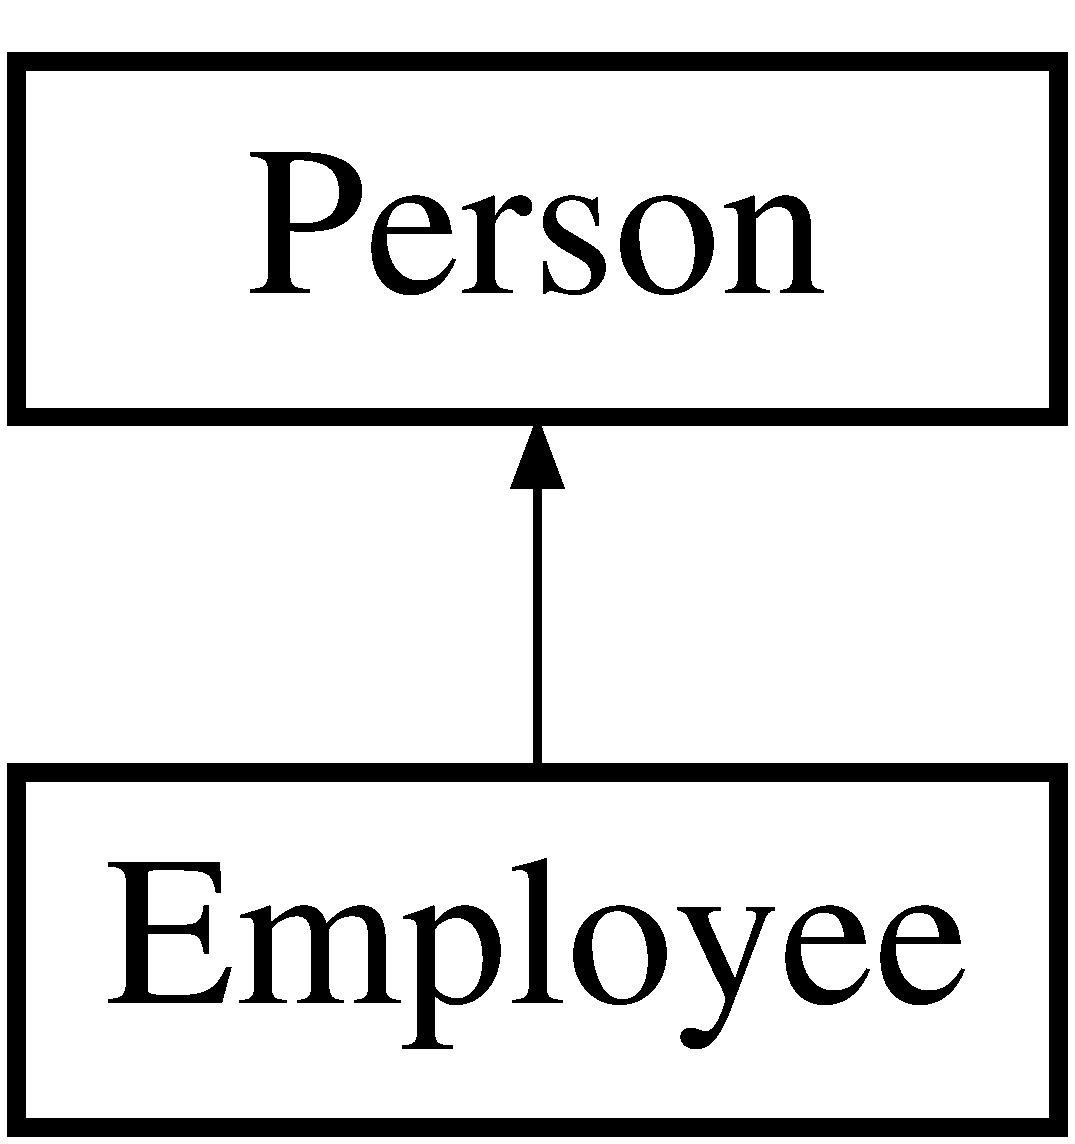
\includegraphics[height=2.000000cm]{class_employee}
\end{center}
\end{figure}
\subsection*{Public Member Functions}
\begin{DoxyCompactItemize}
\item 
\hyperlink{class_employee_a870d18c216c82139c4871ea87c3096a6}{Employee} (int id)
\item 
\hypertarget{class_employee_a69e8f49bccbea1023a0830620a394a2c}{void {\bfseries set\+Payrate} (float)}\label{class_employee_a69e8f49bccbea1023a0830620a394a2c}

\item 
\hypertarget{class_employee_aeeb769c2fdf086f0a3de58764e608913}{void {\bfseries set\+Hours} (float)}\label{class_employee_aeeb769c2fdf086f0a3de58764e608913}

\item 
\hypertarget{class_employee_a4c1a5a5dac43e63f1a80fe5b4c01dbbb}{int {\bfseries get\+Type} ()}\label{class_employee_a4c1a5a5dac43e63f1a80fe5b4c01dbbb}

\item 
\hypertarget{class_employee_a5afdea5fc7e92b5be16f0dac46e02368}{float {\bfseries get\+Payrate} ()}\label{class_employee_a5afdea5fc7e92b5be16f0dac46e02368}

\item 
\hypertarget{class_employee_a6b13934fd60774f89aab4c98b977447b}{float {\bfseries get\+Hours} ()}\label{class_employee_a6b13934fd60774f89aab4c98b977447b}

\item 
\hypertarget{class_employee_a4f05431c08f9bfa4705b3a440b703622}{float {\bfseries get\+Pay} ()}\label{class_employee_a4f05431c08f9bfa4705b3a440b703622}

\item 
string \hyperlink{class_employee_a4357aae7c7ea554889297a93cd3265e8}{to\+String} ()
\end{DoxyCompactItemize}
\subsection*{Additional Inherited Members}


\subsection{Constructor \& Destructor Documentation}
\hypertarget{class_employee_a870d18c216c82139c4871ea87c3096a6}{\index{Employee@{Employee}!Employee@{Employee}}
\index{Employee@{Employee}!Employee@{Employee}}
\subsubsection[{Employee}]{\setlength{\rightskip}{0pt plus 5cm}Employee\+::\+Employee (
\begin{DoxyParamCaption}
\item[{int}]{id}
\end{DoxyParamCaption}
)}}\label{class_employee_a870d18c216c82139c4871ea87c3096a6}
Constructor 
\begin{DoxyParams}{Parameters}
{\em filename} & \\
\hline
\end{DoxyParams}


\subsection{Member Function Documentation}
\hypertarget{class_employee_a4357aae7c7ea554889297a93cd3265e8}{\index{Employee@{Employee}!to\+String@{to\+String}}
\index{to\+String@{to\+String}!Employee@{Employee}}
\subsubsection[{to\+String}]{\setlength{\rightskip}{0pt plus 5cm}string Employee\+::to\+String (
\begin{DoxyParamCaption}
{}
\end{DoxyParamCaption}
)\hspace{0.3cm}{\ttfamily [virtual]}}}\label{class_employee_a4357aae7c7ea554889297a93cd3265e8}
write object to string for saving \begin{DoxyReturn}{Returns}

\end{DoxyReturn}


Implements \hyperlink{class_person}{Person}.



The documentation for this class was generated from the following files\+:\begin{DoxyCompactItemize}
\item 
Employee.\+h\item 
Employee.\+cpp\end{DoxyCompactItemize}

\hypertarget{class_intern}{\section{Intern Class Reference}
\label{class_intern}\index{Intern@{Intern}}
}
Inheritance diagram for Intern\+:\begin{figure}[H]
\begin{center}
\leavevmode
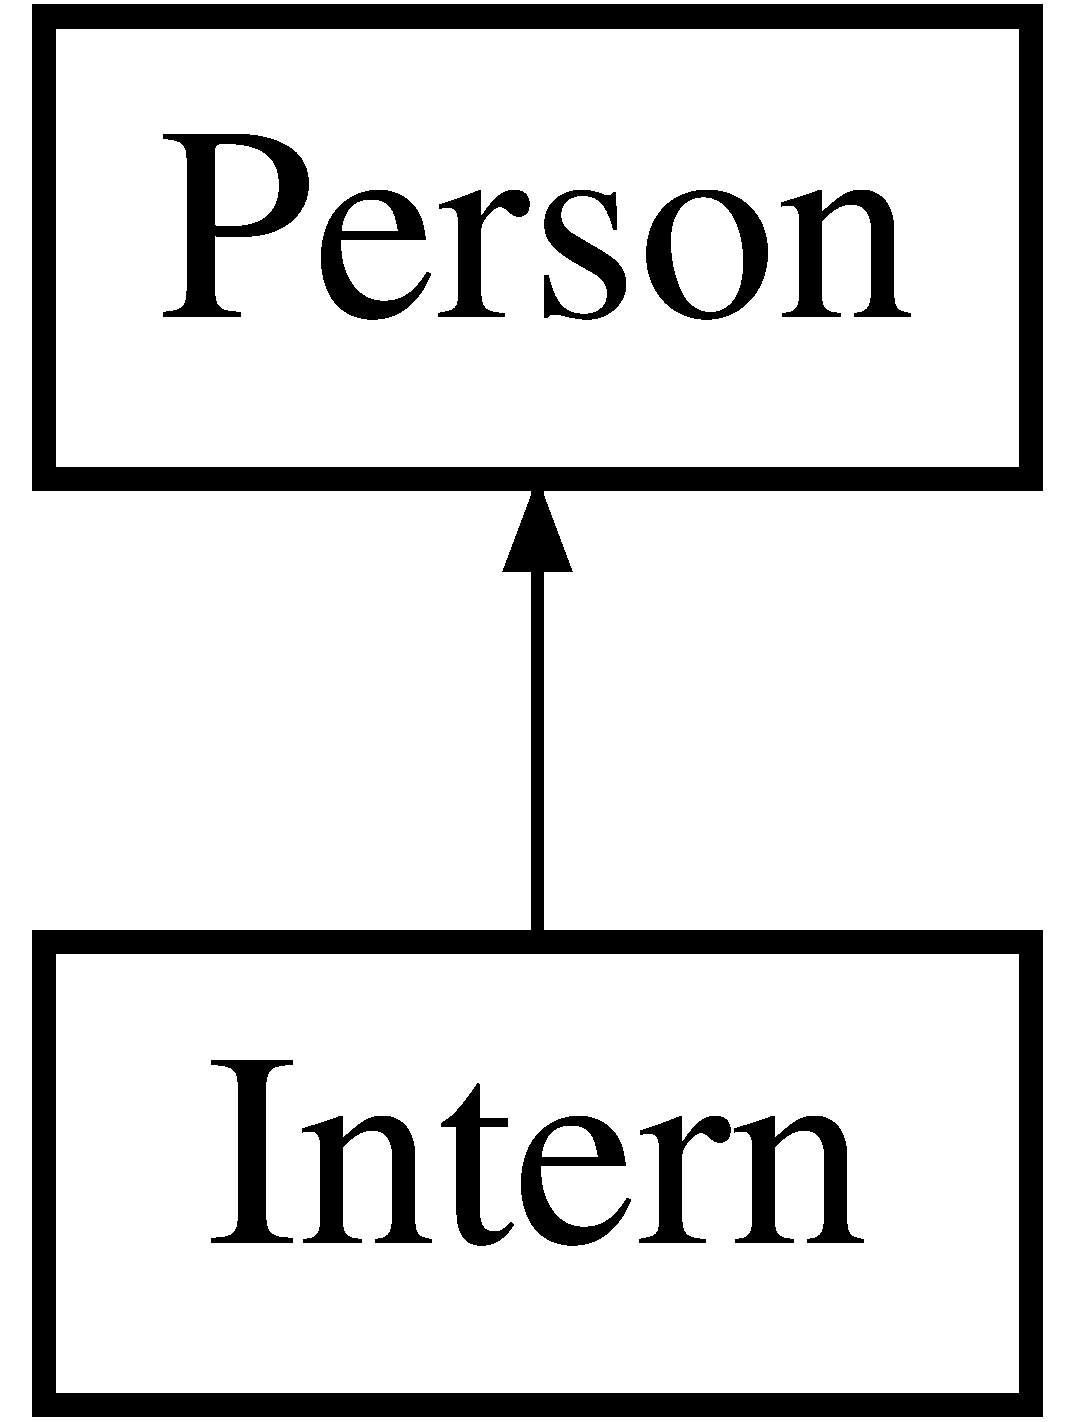
\includegraphics[height=2.000000cm]{class_intern}
\end{center}
\end{figure}
\subsection*{Public Member Functions}
\begin{DoxyCompactItemize}
\item 
\hyperlink{class_intern_adbbfa5e0b5451fb83cd6000e238cbb44}{Intern} (int id=0)
\item 
\hypertarget{class_intern_a04aa681b24ee4ead502a30ad5f2724ad}{void {\bfseries set\+Payrate} (float)}\label{class_intern_a04aa681b24ee4ead502a30ad5f2724ad}

\item 
\hypertarget{class_intern_af783dd0abf31cbb3a57ddb46f6949d54}{void {\bfseries set\+Hours} (float)}\label{class_intern_af783dd0abf31cbb3a57ddb46f6949d54}

\item 
\hypertarget{class_intern_a701018c40635e899355345837b52dee4}{void {\bfseries set\+Is\+Paid} (bool)}\label{class_intern_a701018c40635e899355345837b52dee4}

\item 
\hypertarget{class_intern_af03421c6a2f6e24c4d2429a024cf9df7}{int {\bfseries get\+Type} ()}\label{class_intern_af03421c6a2f6e24c4d2429a024cf9df7}

\item 
\hypertarget{class_intern_a96c0406cc62b6bcbf8373831ea301377}{float {\bfseries get\+Payrate} ()}\label{class_intern_a96c0406cc62b6bcbf8373831ea301377}

\item 
\hypertarget{class_intern_a351faa84f1976a746fee681fce052be7}{float {\bfseries get\+Hours} ()}\label{class_intern_a351faa84f1976a746fee681fce052be7}

\item 
\hypertarget{class_intern_abe81a82954001ff5c52c16da91ae4285}{float {\bfseries get\+Pay} ()}\label{class_intern_abe81a82954001ff5c52c16da91ae4285}

\item 
\hypertarget{class_intern_af4df739723466bc6ab2bb56f008a7fdc}{bool {\bfseries get\+Is\+Paid} ()}\label{class_intern_af4df739723466bc6ab2bb56f008a7fdc}

\item 
string \hyperlink{class_intern_a93797b17f810c7400303f63d9e49fc9a}{to\+String} ()
\end{DoxyCompactItemize}
\subsection*{Additional Inherited Members}


\subsection{Constructor \& Destructor Documentation}
\hypertarget{class_intern_adbbfa5e0b5451fb83cd6000e238cbb44}{\index{Intern@{Intern}!Intern@{Intern}}
\index{Intern@{Intern}!Intern@{Intern}}
\subsubsection[{Intern}]{\setlength{\rightskip}{0pt plus 5cm}Intern\+::\+Intern (
\begin{DoxyParamCaption}
\item[{int}]{id = {\ttfamily 0}}
\end{DoxyParamCaption}
)}}\label{class_intern_adbbfa5e0b5451fb83cd6000e238cbb44}
Constructor 
\begin{DoxyParams}{Parameters}
{\em filename} & \\
\hline
\end{DoxyParams}


\subsection{Member Function Documentation}
\hypertarget{class_intern_a93797b17f810c7400303f63d9e49fc9a}{\index{Intern@{Intern}!to\+String@{to\+String}}
\index{to\+String@{to\+String}!Intern@{Intern}}
\subsubsection[{to\+String}]{\setlength{\rightskip}{0pt plus 5cm}string Intern\+::to\+String (
\begin{DoxyParamCaption}
{}
\end{DoxyParamCaption}
)\hspace{0.3cm}{\ttfamily [virtual]}}}\label{class_intern_a93797b17f810c7400303f63d9e49fc9a}
write object to string for saving \begin{DoxyReturn}{Returns}

\end{DoxyReturn}


Implements \hyperlink{class_person}{Person}.



The documentation for this class was generated from the following files\+:\begin{DoxyCompactItemize}
\item 
Intern.\+h\item 
Intern.\+cpp\end{DoxyCompactItemize}

\hypertarget{class_person}{\section{Person Class Reference}
\label{class_person}\index{Person@{Person}}
}
Inheritance diagram for Person\+:\begin{figure}[H]
\begin{center}
\leavevmode
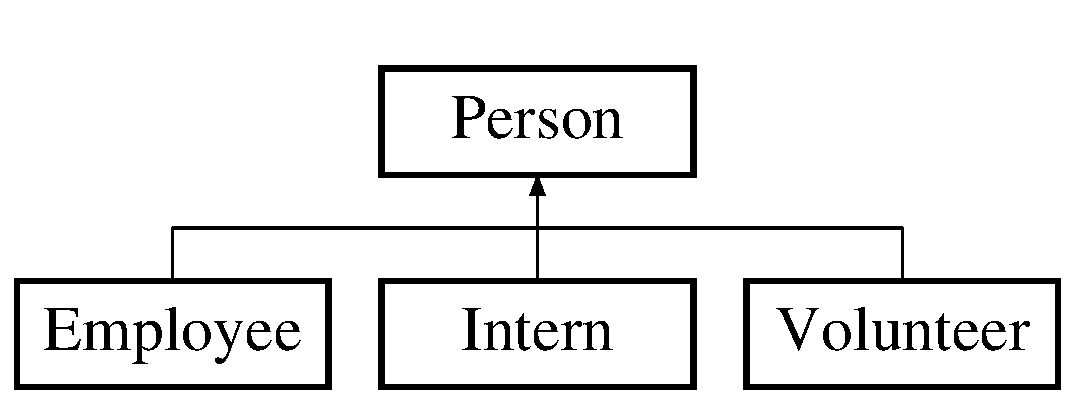
\includegraphics[height=2.000000cm]{class_person}
\end{center}
\end{figure}
\subsection*{Public Member Functions}
\begin{DoxyCompactItemize}
\item 
\hypertarget{class_person_a874693448221e7a4c2c8878dd4f8b876}{void {\bfseries set\+Fname} (string)}\label{class_person_a874693448221e7a4c2c8878dd4f8b876}

\item 
\hypertarget{class_person_a954e69be2153d5fe6858d59a3b46e369}{void {\bfseries set\+Lname} (string)}\label{class_person_a954e69be2153d5fe6858d59a3b46e369}

\item 
\hypertarget{class_person_aa804ae1eb3d21f96b21713da3e1cbe44}{void {\bfseries set\+Id} (int)}\label{class_person_aa804ae1eb3d21f96b21713da3e1cbe44}

\item 
\hypertarget{class_person_a175856114e2790a682702f0c88ec09d8}{void {\bfseries set\+Age} (int)}\label{class_person_a175856114e2790a682702f0c88ec09d8}

\item 
void \hyperlink{class_person_a086666998e8bf5eeb541c1955908415c}{set\+Sex} (int)
\item 
\hypertarget{class_person_ac1c4c72689d7c79f8e70e2411f15e330}{string {\bfseries get\+Fname} ()}\label{class_person_ac1c4c72689d7c79f8e70e2411f15e330}

\item 
\hypertarget{class_person_add2355bbf0eae4c0e2b04b92dc22cd97}{string {\bfseries get\+Lname} ()}\label{class_person_add2355bbf0eae4c0e2b04b92dc22cd97}

\item 
\hypertarget{class_person_a047c1b206440f24865ce6fe8d7685764}{virtual string {\bfseries to\+String} ()=0}\label{class_person_a047c1b206440f24865ce6fe8d7685764}

\item 
\hypertarget{class_person_afd0359228a09c4adcffe31f456046717}{int {\bfseries get\+Id} ()}\label{class_person_afd0359228a09c4adcffe31f456046717}

\item 
\hypertarget{class_person_a69b1611320c68967067747c91783d883}{int {\bfseries get\+Age} ()}\label{class_person_a69b1611320c68967067747c91783d883}

\item 
\hypertarget{class_person_a75d864f8a145630e2383981deeb00a69}{int {\bfseries get\+Sex} ()}\label{class_person_a75d864f8a145630e2383981deeb00a69}

\item 
\hypertarget{class_person_a7e116f792f637be557886a40f0c25289}{char {\bfseries get\+Sex\+Letter} ()}\label{class_person_a7e116f792f637be557886a40f0c25289}

\item 
\hypertarget{class_person_aa814a137ebeded60466a3302d9872976}{virtual int {\bfseries get\+Type} ()=0}\label{class_person_aa814a137ebeded60466a3302d9872976}

\item 
\hypertarget{class_person_a4e12f62a330e97d3c1b06c93072dfcb3}{virtual float {\bfseries get\+Pay} ()=0}\label{class_person_a4e12f62a330e97d3c1b06c93072dfcb3}

\end{DoxyCompactItemize}
\subsection*{Protected Attributes}
\begin{DoxyCompactItemize}
\item 
\hypertarget{class_person_ad309158f21ba32d14c3669c514d10e69}{string {\bfseries fname}}\label{class_person_ad309158f21ba32d14c3669c514d10e69}

\item 
\hypertarget{class_person_ad67a1b71fe9a51dc086fa442efa16761}{string {\bfseries lname}}\label{class_person_ad67a1b71fe9a51dc086fa442efa16761}

\item 
\hypertarget{class_person_aec48a92f614a854ff380a15eb8e2f479}{int {\bfseries id}}\label{class_person_aec48a92f614a854ff380a15eb8e2f479}

\item 
\hypertarget{class_person_acf9db1a60683f40b20ae569d29852d69}{int {\bfseries age}}\label{class_person_acf9db1a60683f40b20ae569d29852d69}

\item 
\hypertarget{class_person_af18f23a4bdcad1283599ed22ab267e0c}{int {\bfseries sex}}\label{class_person_af18f23a4bdcad1283599ed22ab267e0c}

\end{DoxyCompactItemize}


\subsection{Member Function Documentation}
\hypertarget{class_person_a086666998e8bf5eeb541c1955908415c}{\index{Person@{Person}!set\+Sex@{set\+Sex}}
\index{set\+Sex@{set\+Sex}!Person@{Person}}
\subsubsection[{set\+Sex}]{\setlength{\rightskip}{0pt plus 5cm}void Person\+::set\+Sex (
\begin{DoxyParamCaption}
\item[{int}]{s}
\end{DoxyParamCaption}
)}}\label{class_person_a086666998e8bf5eeb541c1955908415c}
set the sex 0 F, 1 M 
\begin{DoxyParams}{Parameters}
{\em s} & \\
\hline
\end{DoxyParams}


The documentation for this class was generated from the following files\+:\begin{DoxyCompactItemize}
\item 
Person.\+h\item 
Person.\+cpp\end{DoxyCompactItemize}

\hypertarget{class_volunteer}{\section{Volunteer Class Reference}
\label{class_volunteer}\index{Volunteer@{Volunteer}}
}
Inheritance diagram for Volunteer\+:\begin{figure}[H]
\begin{center}
\leavevmode
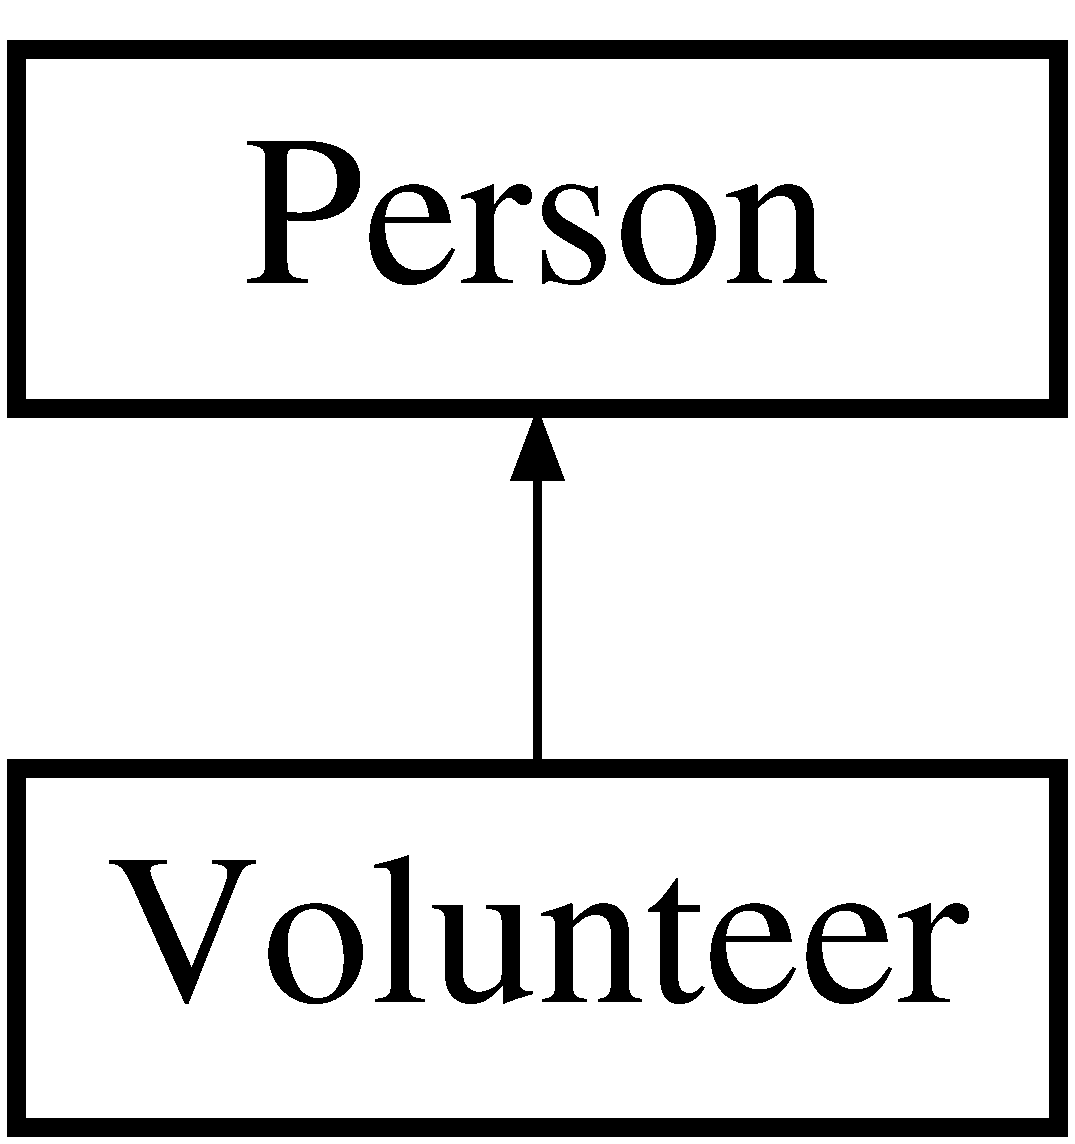
\includegraphics[height=2.000000cm]{class_volunteer}
\end{center}
\end{figure}
\subsection*{Public Member Functions}
\begin{DoxyCompactItemize}
\item 
\hyperlink{class_volunteer_a33cb19b8511035c139c6015eef4a20d3}{Volunteer} (int)
\item 
\hypertarget{class_volunteer_a927b7a0d08617bc1fc8227a8eed97904}{void {\bfseries set\+Hours} (float)}\label{class_volunteer_a927b7a0d08617bc1fc8227a8eed97904}

\item 
\hypertarget{class_volunteer_a855153a69c8ab88048e7f51a5f837c7a}{int {\bfseries get\+Type} ()}\label{class_volunteer_a855153a69c8ab88048e7f51a5f837c7a}

\item 
\hypertarget{class_volunteer_a8fa1b19a352f0c96a2de4e98960f6a6e}{float {\bfseries get\+Hours} ()}\label{class_volunteer_a8fa1b19a352f0c96a2de4e98960f6a6e}

\item 
\hypertarget{class_volunteer_a8df05e8e35d2f0c31fe64ea7803b3620}{float {\bfseries get\+Pay} ()}\label{class_volunteer_a8df05e8e35d2f0c31fe64ea7803b3620}

\item 
string \hyperlink{class_volunteer_aa5dcc7c3680a1690edbb0ee36dbb002b}{to\+String} ()
\end{DoxyCompactItemize}
\subsection*{Additional Inherited Members}


\subsection{Constructor \& Destructor Documentation}
\hypertarget{class_volunteer_a33cb19b8511035c139c6015eef4a20d3}{\index{Volunteer@{Volunteer}!Volunteer@{Volunteer}}
\index{Volunteer@{Volunteer}!Volunteer@{Volunteer}}
\subsubsection[{Volunteer}]{\setlength{\rightskip}{0pt plus 5cm}Volunteer\+::\+Volunteer (
\begin{DoxyParamCaption}
\item[{int}]{id}
\end{DoxyParamCaption}
)}}\label{class_volunteer_a33cb19b8511035c139c6015eef4a20d3}
Constructor 
\begin{DoxyParams}{Parameters}
{\em filename} & \\
\hline
\end{DoxyParams}


\subsection{Member Function Documentation}
\hypertarget{class_volunteer_aa5dcc7c3680a1690edbb0ee36dbb002b}{\index{Volunteer@{Volunteer}!to\+String@{to\+String}}
\index{to\+String@{to\+String}!Volunteer@{Volunteer}}
\subsubsection[{to\+String}]{\setlength{\rightskip}{0pt plus 5cm}string Volunteer\+::to\+String (
\begin{DoxyParamCaption}
{}
\end{DoxyParamCaption}
)\hspace{0.3cm}{\ttfamily [virtual]}}}\label{class_volunteer_aa5dcc7c3680a1690edbb0ee36dbb002b}
write object to string for saving \begin{DoxyReturn}{Returns}

\end{DoxyReturn}


Implements \hyperlink{class_person}{Person}.



The documentation for this class was generated from the following files\+:\begin{DoxyCompactItemize}
\item 
Volunteer.\+h\item 
Volunteer.\+cpp\end{DoxyCompactItemize}

%--- End generated contents ---

% Index
\newpage
\phantomsection
\addcontentsline{toc}{chapter}{Index}
\printindex

\end{document}
